\documentclass[]{jarticle}          % 一段組
%\documentclass[twocolumn]{jarticle} % 二段組

\textwidth 180mm
\textheight 255mm
\oddsidemargin -12mm
\topmargin -15mm
\columnsep 10mm

%\vspace{0.5cm} % 一段組の場合はコメントアウトした方が体裁がよいx
%] % 一段組の場合はコメントアウトする

\usepackage{styles/labheadings}
\usepackage[dvipdfmx]{graphicx,color}
\usepackage{amsmath,amssymb}
\usepackage{url}
% 追加
\usepackage{listings,jvlisting} 
\usepackage[hang,small,bf]{caption}
\usepackage[subrefformat=parens]{subcaption}
\usepackage{indentfirst}
\captionsetup{compatibility=false}

\newcommand{\aU}{\mbox{\boldmath $a$}}
\newcommand{\bU}{\mbox{\boldmath $b$}}
\newcommand{\cU}{\mbox{\boldmath $c$}}
\newcommand{\dU}{\mbox{\boldmath $d$}}
\newcommand{\eU}{\mbox{\boldmath $e$}}
\newcommand{\fU}{\mbox{\boldmath $f$}}
\newcommand{\gU}{\mbox{\boldmath $g$}}
\newcommand{\hU}{\mbox{\boldmath $h$}}
\newcommand{\iU}{\mbox{\boldmath $i$}}
\newcommand{\jU}{\mbox{\boldmath $j$}}
\newcommand{\kU}{\mbox{\boldmath $k$}}
\newcommand{\lU}{\mbox{\boldmath $l$}}
\newcommand{\mU}{\mbox{\boldmath $m$}}
\newcommand{\nU}{\mbox{\boldmath $n$}}
\newcommand{\oU}{\mbox{\boldmath $o$}}
\newcommand{\pU}{\mbox{\boldmath $p$}}
\newcommand{\qU}{\mbox{\boldmath $q$}}
\newcommand{\rU}{\mbox{\boldmath $r$}}
\newcommand{\sU}{\mbox{\boldmath $s$}}
\newcommand{\tU}{\mbox{\boldmath $t$}}
\newcommand{\uU}{\mbox{\boldmath $u$}}
\newcommand{\vU}{\mbox{\boldmath $v$}}
\newcommand{\wU}{\mbox{\boldmath $w$}}
\newcommand{\xU}{\mbox{\boldmath $x$}}
\newcommand{\yU}{\mbox{\boldmath $y$}}
\newcommand{\zU}{\mbox{\boldmath $z$}}
\newcommand{\AU}{\mbox{\boldmath $A$}}
\newcommand{\BU}{\mbox{\boldmath $B$}}
\newcommand{\CU}{\mbox{\boldmath $C$}}
\newcommand{\DU}{\mbox{\boldmath $D$}}
\newcommand{\EU}{\mbox{\boldmath $E$}}
\newcommand{\FU}{\mbox{\boldmath $F$}}
\newcommand{\GU}{\mbox{\boldmath $G$}}
\newcommand{\HU}{\mbox{\boldmath $H$}}
\newcommand{\IU}{\mbox{\boldmath $I$}}
\newcommand{\JU}{\mbox{\boldmath $J$}}
\newcommand{\KU}{\mbox{\boldmath $K$}}
\newcommand{\LU}{\mbox{\boldmath $L$}}
\newcommand{\MU}{\mbox{\boldmath $M$}}
\newcommand{\NU}{\mbox{\boldmath $N$}}
\newcommand{\OU}{\mbox{\boldmath $O$}}
\newcommand{\PU}{\mbox{\boldmath $P$}}
\newcommand{\QU}{\mbox{\boldmath $Q$}}
\newcommand{\RU}{\mbox{\boldmath $R$}}
\newcommand{\SU}{\mbox{\boldmath $S$}}
\newcommand{\TU}{\mbox{\boldmath $T$}}
\newcommand{\UU}{\mbox{\boldmath $U$}}
\newcommand{\VU}{\mbox{\boldmath $V$}}
\newcommand{\WU}{\mbox{\boldmath $W$}}
\newcommand{\XU}{\mbox{\boldmath $X$}}
\newcommand{\YU}{\mbox{\boldmath $Y$}}
\newcommand{\ZU}{\mbox{\boldmath $Z$}}
\newcommand{\epU}{\mbox{\boldmath $\epsilon$}}
\newcommand{\taU}{\mbox{\boldmath $\tau$}}
\newcommand{\etU}{\mbox{\boldmath $\eta$}}
\newcommand{\xiU}{\mbox{\boldmath $\xi$}}
\newcommand{\wwU}{\mbox{\boldmath $\omega$}}
\newcommand{\WwU}{\mbox{\boldmath $\Omega$}}
\newcommand{\lmU}{\mbox{\boldmath $\lambda$}}
\newcommand{\LmU}{\mbox{\boldmath $\Lambda$}}
\newcommand{\PiU}{\mbox{\boldmath $\Pi$}}
\newcommand{\SgU}{\mbox{\boldmath $\Sigma$}}
\newcommand{\thU}{\mbox{\boldmath $\theta$}}
\newcommand{\ThU}{\mbox{\boldmath $\Theta$}}
\newcommand{\roU}{\mbox{\boldmath $\rho$}}
\newcommand{\nuU}{\mbox{\boldmath $\nu$}}
\newcommand{\ones}{{\bf 1}}
\newcommand{\zr}{{\bf 0}}
\newcommand{\eq}{\begin{equation}}
\newcommand{\en}{\end{equation}}
\newcommand{\eqa}{\begin{eqnarray}}
\newcommand{\ena}{\end{eqnarray}}
\newcommand{\xx}{\makebox[1cm]{}}
\newcommand{\xm}{\makebox[0.5cm]{}}
\newcommand{\x}{\makebox[0.2cm]{}}
\newcommand{\tr}{{\rm tr}}
\newcommand{\sgn}{{\rm sgn}}
\newcommand{\ad}{{\rm ad}}

\newcommand{\rank}{{\rm rank}}
\newcommand{\diag}{{\rm diag}}
\newcommand{\lbr}{\left(\begin{array}}
\newcommand{\rbr}{\end{array}\right)}
\newcommand{\Proof}{\noindent{\em Proof\/}}
\newcommand{\Solution}{\noindent{\em Solution}}
\newcommand{\Derivation}{\noindent{\em Derivation}}
\newcommand{\msp}{\vspace*{\medskipamount}\\}
\newcommand{\qed}{\hspace*{\fill}$\Box$}
\newcommand{\aX}{{\bf a}}
\newcommand{\bX}{{\bf b}}
\newcommand{\cX}{{\bf c}}
\newcommand{\dX}{{\bf d}}
\newcommand{\eX}{{\bf e}}
\newcommand{\fX}{{\bf f}}
\newcommand{\gX}{{\bf g}}
\newcommand{\hX}{{\bf h}}
\newcommand{\iX}{{\bf i}}
\newcommand{\jX}{{\bf j}}
\newcommand{\kX}{{\bf k}}
\newcommand{\lX}{{\bf l}}
\newcommand{\mX}{{\bf m}}
\newcommand{\nX}{{\bf n}}
\newcommand{\oX}{{\bf o}}
\newcommand{\pX}{{\bf p}}
\newcommand{\qX}{{\bf q}}
\newcommand{\rX}{{\bf r}}
\newcommand{\sX}{{\bf s}}
\newcommand{\tX}{{\bf t}}
\newcommand{\uX}{{\bf u}}
\newcommand{\vX}{{\bf v}}
\newcommand{\wX}{{\bf w}}
\newcommand{\xX}{{\bf x}}
\newcommand{\yX}{{\bf y}}
\newcommand{\zX}{{\bf z}}
\newcommand{\AX}{{\bf A}}
\newcommand{\BX}{{\bf B}}
\newcommand{\CX}{{\bf C}}
\newcommand{\DX}{{\bf D}}
\newcommand{\EX}{{\bf E}}
\newcommand{\FX}{{\bf F}}
\newcommand{\GX}{{\bf G}}
\newcommand{\HX}{{\bf H}}
\newcommand{\IX}{{\bf I}}
\newcommand{\JX}{{\bf J}}
\newcommand{\KX}{{\bf K}}
\newcommand{\LX}{{\bf L}}
\newcommand{\MX}{{\bf M}}
\newcommand{\NX}{{\bf N}}
\newcommand{\OX}{{\bf O}}
\newcommand{\PX}{{\bf P}}
\newcommand{\QX}{{\bf Q}}
\newcommand{\RX}{{\bf R}}
\newcommand{\SX}{{\bf S}}
\newcommand{\TX}{{\bf T}}
\newcommand{\UX}{{\bf U}}
\newcommand{\VX}{{\bf V}}
\newcommand{\WX}{{\bf W}}
\newcommand{\XX}{{\bf X}}
\newcommand{\YX}{{\bf Y}}
\newcommand{\ZX}{{\bf Z}}

% report.texと同じディレクトリにnumerical_definition.texを入れておけば上の書き方でもいいはずです

\usepackage[
  dvipdfm,
  bookmarks=true,
  bookmarksnumbered=true,
  colorlinks=true]{hyperref}
\AtBeginDvi{\special{pdf:tounicode EUC-UCS2}}

%ここからソースコードの表示に関する設定
\lstset{
  basicstyle={\ttfamily},
  identifierstyle={\small},
  commentstyle={\smallitshape},
  keywordstyle={\small\bfseries},
  ndkeywordstyle={\small},
  stringstyle={\small\ttfamily},
  frame={tb},
  breaklines=true,
  columns=[l]{fullflexible},
  numbers=left,
  xrightmargin=0zw,
  xleftmargin=3zw,
  numberstyle={\scriptsize},
  stepnumber=1,
  numbersep=1zw,
  lineskip=-0.5ex
}
%ここまでソースコードの表示に関する設定

\pagestyle{labheadings}
\headerleft{課題1}   % ヘッダの左側のタイトル
\headerright{2024年5月1日}  % ヘッダの右側のタイトル

\begin{document}

%\twocolumn % 一段組の場合はコメントアウトする

\vspace*{2ex}
\begin{center}
 {\Large \bf 数値解析・最適化工学特論 課題1}\\ % タイトル
 \vspace*{5mm}
 {\large M1 田川幸汰}% 発表者名
\end{center}

%\vspace{0.5cm} % 一段組の場合はコメントアウトした方が体裁がよいx
%] % 一段組の場合はコメントアウトする

%新しく作成したコマンド
% \newcommand{\reffig}[1]{\hyperref[#1]{図\ref{#1}}}
% \newcommand{\refeq}[1]{\hyperref[#1]{式(\ref{#1})}}
% \newcommand{\reftab}[1]{\hyperref[#1]{表\ref{#1}}}
% \newcommand{\refsec}[1]{\hyperref[#1]{\ref{#1}章}}
% \newcommand{\refsubsec}[1]{\hyperref[#1]{\ref{#1}節}}

\section{課題1}
$J=\sum_{a=1}^{N}(x_a-\bar{x_a}, V[x_a]=^{-1}(x_a-\bar{x_a}))$からラグランジュの未定乗数法を用いて$\bar{x_a}$を求め、次の関数を導出しなさい。
\begin{equation}
  J = \sum_{a=1}^{N}\frac{(x_a,u)^2}{(u,V[x_a]u)}
\end{equation}

\subsection{解答}
真の値のデータを$\bar{x_a}$、誤差を含むデータを$x_a$とすると、その誤差$\Delta{x_a}$は$x_a-\bar{x_a}$で表される。
$u$をパラメータベクトルとして含む際の制約条件$g(x_a)$は式(\ref{two})で表される。
\begin{equation}
  g(x_a)=(\bar{x_a},u)=(x_a-\Delta{x_a},u)=0, a=1,...,N
  \label{two}
\end{equation}

与式に$\bar{x_a}=x_a-\Delta{x_a}$を代入すると式(\ref{three})が得られる。
\begin{equation}
  J = \sum_{a=1}^{N}(x_a-(x_a-\Delta{x_a}),V[x_a]^{-1}x_a-(x_a-\Delta{x_a}))=\sum_{a=1}^{N}(\Delta{x_a},V[x_a]^{-1}\Delta{x_a})
  \label{three}
\end{equation}

式(\ref{two})で求めた制約条件$g(x_a)$と式(\ref{three})=$f(x_a)$を用いて、ラグランジュの未定乗数法を計算すると式(\ref{four})が得られる。
\begin{equation}
  F(x_a,\lambda)=f(x_a)-\lambda{g(x_a)}=\sum_{a=1}^{N}(\Delta{x_a},V[x_a]^{-1}\Delta{x_a})-\sum_{a=1}^{N}\lambda_a(x_a-\Delta{x_a},u)
  \label{four}
\end{equation}

式(\ref{four})の$\Delta{x_a}$に関する偏微分は式(\ref{five})で表される。ここで、式(\ref{four})の第一項は二次形式、第二項は内積の偏微分を計算する。
また、式(\ref{four})の$\lambda_a$に関する偏微分は式(\ref{six})で表される。第一項は$\lambda_a$を含まないため0となる。
\begin{equation}
  \frac{\delta}{\delta\Delta{x_a}}F(x_a,\lambda)=2V[x_a]-{-1}\Delta{x_a}-\lambda_a{u}=0
  \label{five}
\end{equation}

\begin{equation}
  \frac{\delta}{\delta\lambda_a}F(x_a,\lambda)=(x_a-\Delta{x_a},u)=0
  \label{six}
\end{equation}

式(\ref{five})から$\Delta{x_a}$は式(\ref{seven})で表される。
\begin{equation}
  \Delta{x_a}=\frac{\lambda_a}{2}V[x_a]u
  \label{seven}
\end{equation}

式(\ref{six})と式(\ref{seven})を用いて、$\lambda_a$は式(\ref{eight})で表される。
\begin{equation}
  \begin{split}
  (x_a-\frac{\lambda_a}{2}V[x_a]u,u) = 0 \\
  \lambda_a = \frac{2(u,x_a)}{u,V[x_a]u}
  \end{split}
  \label{eight}
\end{equation}

式(\ref{three})に、式(\ref{seven})で求めた$\Delta{x_a}$と式(\ref{eight})で求めた$\lambda_a$を代入すると、式(\ref{nine})が得られる。
\begin{equation}
  \begin{split}
    J &= \sum_{a=1}^{N}(\frac{\lambda_a}{2}V[x_a]u,V[x_a]^{-1}\frac{\lambda_a}{2}V[x_a]u) \\
    &= \frac{1}{4}\sum_{a=1}^{N}\lambda_a^2(V[x_a]u,u) \\
    &= \frac{1}{4}\sum_{a=1}^{N}(\frac{2(u,x_a)}{(u,V[x_a]u)})^2(V[x_a]u,u) \\
    &= \frac{1}{4}\sum_{a=1}^{N}\frac{4(u,x_a)^2}{(u,V[x_a]u)^2}(V[x_a]u,u) \\
    &= \sum_{a=1}^{N}\frac{(u,x_a)^2}{(u,V[x_a]u)} \\
  \end{split}
  \label{nine}
\end{equation}

式(\ref{nine})より、$J = \sum_{a=1}^{N}\frac{(x_a,u)^2}{(u,V[x_a]u)}$となる。

\section{課題2}
$x=300\cos\theta$, $y=200\sin\theta$で表される楕円状の点列$(x_i,y_i)$を次のように生成しなさい。また、生成した点列を描画してその分布を確認しなさい。
\begin{equation}
  (x_i,y_i)=(300\cos\theta_i, 200\sin\theta_i),\quad \theta_i = - \frac{\pi}{4}+\frac{11\pi}{12N}i,\quad i = 0,...,N-1
\end{equation}
\subsection{解答}
$N=100$として生成した楕円を図\ref{figone}に示す。
\begin{figure}[!ht]
  \begin{center}
    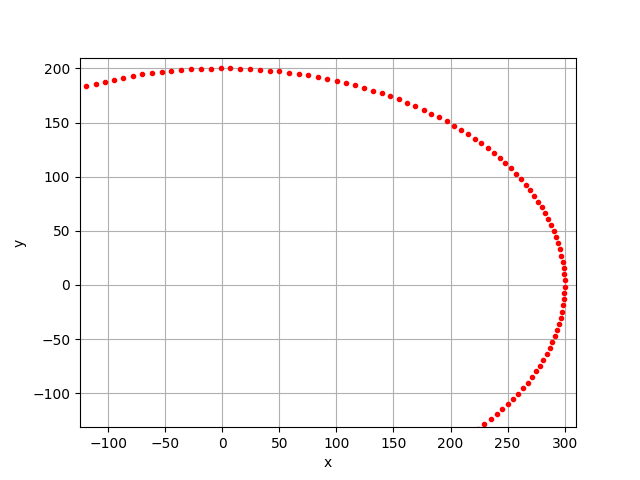
\includegraphics[keepaspectratio, width=0.7\linewidth]{figures/kadai2.png}
  \end{center}
  \caption{楕円}
  \label{figone}
\end{figure}

中心が$(x,y)=(0,0)$、$X$軸方向に300、$Y$軸方向に200、傾き0の楕円上の100点が描画されている。

\section{課題3}
課題2で生成した点列の$x$座標、$y$座標にそれぞれ独立に、平均$\mu = 0$、標準偏差$\sigma = 3.0$の
正規分布に従う誤差を加えたデータを作成しなさい。それを確認するために課題2の描画結果と重ねて描画しなさい。
\subsection{解答}
$N=100$として誤差を加えた点と真値の点を重ねた楕円を図\ref{figtwo}に示す。
\begin{figure}[!ht]
  \begin{center}
    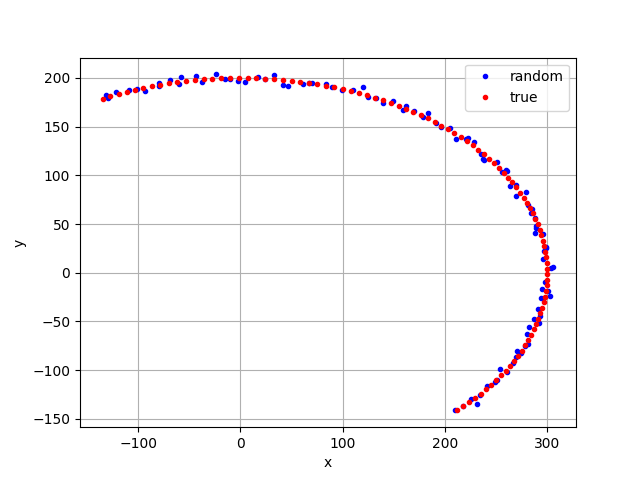
\includegraphics[keepaspectratio, width=0.7\linewidth]{figures/kadai3.png}
  \end{center}
  \caption{誤差を加えた楕円}
  \label{figtwo}
\end{figure}

赤色の点が真値の点、青色の点が$x$座標、$y$座標にそれぞれ独立に、平均$\mu = 0$、標準偏差$\sigma = 3.0$の
正規分布に従う誤差を加えた点である。

\section{課題4}
課題3の$\sigma$の値を0.1から$\sigma_{max}$まで0.1刻みで変化させたデータを作成し、そのデータに対して
最小2乗法と最尤推定法によって楕円のパラメータを推定しなさい。
このとき、同一の$\sigma$の値に対して異なる誤差を付加したデータを1000回生成してパラメータを推定し、
RMS誤差を計算して、横軸に$\sigma$の値、縦軸にRMS誤差としたグラフを描画しなさい。
ただし、$\sigma_{max}$の値は適切と思われる値を自分で設定しなさい。

\subsection{解答}
楕円の方程式のデータベクトル$xi$を$(x^2 2xy y^2 2x 2y 1)^\top$と定義する。
また、$x$座標、$y$座標にそれぞれ独立に、期待値0、標準偏差$\sigma$の誤差が加わるときの共分散行列を$V[\xi]$とする。
最小二乗法では式(\ref{ten})の最小固有値に対する固有ベクトルを求めることでパラメータを推定する。
\begin{equation}
  M = \sum^N_{a=1}\xi_a\xi_a^{\top}
  \label{ten}
\end{equation}

最尤推定法では目的関数$J$をパラメータベクトル$u$で微分して得られた式(\ref{eleven})で、
$u$の初期値を与えて行列$M,N$を計算することで固有値問題を解き、$u$を更新する反復解法によって解を計算する。
なお、$\uU$の変化量が$10^{-6}$になるまで計算した。
\begin{equation}
  \begin{split}
    \frac{\sigma{f}}{\sigma{\uU}}&=2(\sum^N_{a=1}\frac{\xi_a\xi_a^{\top}}{(\uU,V[\xi_a]\uU)}-\sum^N_{a=1}\frac{(\xi_a,\uU)^2V[\xi_a]}{(\uU,V[\xi_a]\uU)^2})\uU\\
    &=2(\MU-\LU)\uU=0
  \end{split}
  \label{eleven}
\end{equation}

RMS誤差は式(\ref{twelve})で求められる。ここで、$\bar{\uU}$は解の真値、
$\uU^{(i)}$は$i$回目の試行で得た解の推定値を表す。
\begin{equation}
  RMS = \sqrt{\frac{1}{N}\sum^N_{a=1}||(I-\bar{\uU}\bar{\uU}^{\top})\uU^{(i)}||^2}
  \label{twelve}
\end{equation}

$\sigma_{max}=3.0$として、最小2乗法と最尤推定法によって楕円のパラメータを推定した結果を図\ref{figthree}に示す。
\begin{figure}[!ht]
  \begin{center}
    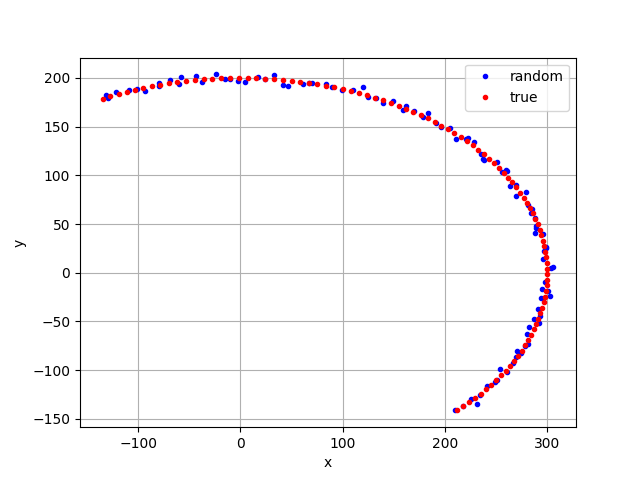
\includegraphics[keepaspectratio, width=0.7\linewidth]{figures/kadai3.png}
  \end{center}
  \caption{誤差を加えた楕円}
  \label{figthree}
\end{figure}

\end{document}
